\documentclass[lettersize,journal]{IEEEtran}
\usepackage{amsmath,amsfonts}
\usepackage{algorithmic}
\usepackage{algorithm}
\usepackage{array}
\usepackage[caption=false,font=normalsize,labelfont=sf,textfont=sf]{subfig}
\usepackage{textcomp}
\usepackage{stfloats}
\usepackage{url}
\usepackage{verbatim}
\usepackage{graphicx}
\graphicspath{{fig/}}
\usepackage{hyperref}
\newtheorem{theorem}{Theorem}
\newtheorem{lemma}{Lemma}[theorem]
\newtheorem{definition}{Definition}
\hyphenation{op-tical net-works semi-conduc-tor IEEE-Xplore}
% updated with editorial comments 8/9/2021

\begin{document}

\title{Anonymous Multi-Factor Authentication Scheme based on Pseudo-Random MSISDN}
\author{Jia Cao, Jianan Hong, Jiayue Zhou, Cunqing Hua}

\maketitle

\begin{abstract}
Multi-factor authentication is a promising technology to improve the security strength of authentication. It is most convenient to achieve that goal by combining the key-based authentication and verification code transferred by short message service (SMS). As the former factor has sufficient algorithms for choice from cryptographic area based on different requirements; and the latter one is easy to deploy since each identity (even device) owns a unique mobile number (MSISDN) to receive text secretly. However, the SMS verification code method reveals user's identity to others, even the key-based method is privacy-preserving algorithm.

This paper focuses on this challenge and proposes a high security-level anonymous authentication scheme. In our scheme, an authentication is executed with the factor of anonymous credential (with BBS+ signature) and the ownership of a valid MSISDN. The used zero-knowledge proof algorithm and designed protocol well tackle relevant issues, two of which are the most technical: 1) the combination is effective, such that the verifier can check whether the MSISDN is valid directly from the attribute from credential factor; 2) The factor of valid MSISDN will not release one bit more privacy other than the showing of anonymous credential. We implement our scheme in the 5G core testbed with Open5GS and USRP devices. The further experimental results and security proof show the advantageous features in terms of security and efficiency.
\end{abstract}

\begin{IEEEkeywords}
Anonymous authentication, multi-factor, zero-knowledge proof, pseudo-random MSISDN.
\end{IEEEkeywords}

\section{Introduction}

%% Background of target technology (MFA or authentication, or cryptographic authentication, or anonymous credential)
\IEEEPARstart{T}{he} advances in network technologies from the architecture (e.g., 5th-generation network, Internet of Things) has resulted in the continuous growth in the numbers of connected smart devices through the Internet, which brings in larger and larger market for organizations and enterprises to provide up-layer network services. As these services trend to offer more valuable or private information data (such as personal balance in a bank, private status of the owner's house), and some services are critical to user's safety (like payment), thus the service should be offered with a well-deployed authentication method to resist various adversaries.
%Large amount of data, possibly relevant to every area of human activity, both public and private, will be produced, communicated, gathered, stored, and processed. To keep the transmitted data safe, authentication acts as the first line of defence against adversaries.

According to [], through the process of authentication, a security system validates whether a user could be granted the corresponding access privilege. Based on the authentication mechanism used, the user provides pieces of evidence (factors) of identity so that the security system is convinced whether the user is who it claims to be, or belongs to a certain legitimate user group. Depend on the specific evidence submitted by the user, authentication factors could be categorized into three groups: knowledge factors, ownership factors, and inherent factors. The knowledge factor is something that only the user knows, such as its password or secret key. The possession factor is something that a user has, such as smart cards or mobile phones. The inherent factor refers to something that qualifies a user, such as biometric data. 
%The location factor refers to somewhere the user is, such as current location or time information. 
In some cases, authentication mechanisms could be integrated with cryptography-defined concepts to expand various functions. For example, the cryptographic challenge-response based authentication protocol is an improvement to privacy of the basic password authentication protocol in terms of brute force and dictionary attacks; By employing attribute-based cryptographic framework, one can realize fine-grained access control of data and resources; The anonymous credential system provides privacy-preservation for user attributes and behaviors and unlinkability under a single sign-on framework. 

``Authentication technologies can both advance and undermine privacy interests'' (National Research Council. 2003). An authentication system may require users to reveal identifying personal information to prove their validity, and the act of authentication itself may be recorded and linked with other user behaviors, causing privacy concerns \cite{national2003goes}. Instead of revealing identifiable information, privacy-concerned users may hope to finish authentication step with a service provider only by showing user's belonging to a valid group or by proving its possession of some specific attribute identifiers\cite{holt2002selective}. Anonymous credential system (ACS) is an effective solution to problem of linkability. Users are known to service providers by pseudonyms in such systems, which ensures the anonymity and unlinkability of authentication[]. In addition, ACS enables privacy-preserving single sign-on (SSO)[]. In traditional SSO, a third party identity provider (IdP) serves as single point of failure; And users are at risk of having their activities tracked by the IdP. On contrary, the process of user authentication no longer depends on a single trusted third party in privacy-preserving SSO[]. In []'s work, the anonymous credential system (ACS) is extended to an attribute-based anonymous credential system (ABACS). Compared to ACS, ABACS enables flexible attribute-based access control and minimal disclosure of information, and is thus welcomed by privacy-concerned users.

Key-based (cryptographic) authentication exhibits fragility in the face of key compromise attacks. Multi-factor authentication overcomes this risk. By requiring more than one factor to authenticate a user, the multi-factor authentication (MFA) makes the intruding process more difficult for hackers, thus providing additional layers of security. For example, MFA used on top of username/password authentication may require users to take an extra step such as entering a code sent to a physical device. Even if the perpetrator brute forces the password, it is not able to get pass the second authentication step without possession of the device. Up till now, few researches has been made on the implementation of ABACS with MFA. The popularization of smartphones has lead to increased usage of short message service (SMS) based multi-factor authentication. In these days, most internet applications require users to accomplish the SMS authentication step to get registered or authenticated, making combination user-friendly. However, one concern is that SMS authentication requires users to transmit their personal information to the service provider, including the user's mobile phone number, which identifies a user's identity better than its real name in today's world. Besides, using the same phone number for each authentication risks damaging the unlinkability provided by ABACS. 

\subsection{Our Contribution}

To address the above problems, we construct a multi-factor authentication scheme that combine attribute-based anonymous credential system with SMS-verification code authentication which employs virtual mobile phone number to protect user privacy. We alter the 5G signalling so that a user who has registered for an SMS-relay service at the 5G system network with a virtual mobile phone number could receive the SMS-verification code on its own mobile phone. When the user wants to authenticate with a service provider (SP), it sends to SP information unique to the user with the mobile phone number replaced by a virtual one. Subsequently, the user's phone number is never transmitted onto the internet.

Our scheme realizes an asynchronous SSO system based on an attribute-based anonymous credential framework. The generation of the material for authentication (the attribute-based credential and related information) is decoupled in time with the process of user's authentication at service provider. Hence relying party (the service provider) no longer has to visit the IdP for identity verification. The IdP could be offline while the authentication process running smoothly, and the tracking of user's activities by IdP is prohibited. The ABACS and the employment of virtual mobile phone number provides solid anonymity and unlinkability.

For many online services, intra-service unlinkability is undesirable. If the generation and registration of virtual phone number is arbitrary, a user may have unlimited number of pseudonyms without restriction. 
In our scheme, the generation of virtual mobile phone number and its registration at the 5G system network are designed to be bounded by the unique identifier of the target service provider.
The user could generate multiple virtual numbers once it has acquired an attribute-based credential, but could not generate and register more than one for the same service provider. 




% If a user consistently uses the same identifier, whether it is a real identity or an anonymous one, to participate in transactions with multiple service providers, it risks exposing its behavioral privacy to the outside. The protection of behavioral privacy has become an important topic in information security. In the age of big data, it is technically possible to accurately analyze users' preferences and interests after mining a large amount of users' continuous behaviors, and to predict the future behavior of users with high accuracy. More dangerously, if an adversary already has acquired a part of the behavior information of an observed entity, and compares it with the behavior data of a de-identified identity, the identity of all behaviors of the user may be recovered, which means that the identity privacy of users would be affected to a certain extent. A core requirement to protect behavioral privacy is to achieve unlinkability in multiple user authentications. That is, if two authentication requests are collected, there is no way to tell whether the two requests are from the same user. In our scheme, inter-service unlinkability is desired. The cancellation of interaction with IdP in the authentication process prevents the IdP from tracking user's activities and different RPs. In addition to this, we hope that the correlation of user's authentication with different RPs should be impossible for any other entities in the system. This implies the unlinkability between user's generated random mobile phone numbers for differents RPs and the unlinkability between the assertion constructed by the user for different RPs.


%Network technologies have been advancing rapidly in recent years from the architecture to the up-layer services, such as fifth-generation (5G) radio network and Internet of Things (IoT). The service-based architecture of 5G network and network slicing technique make it easy to converge high-throughput MBB, low-delay IoT and "ultra-reliable low latency communications (URLLC)" into one system, which significantly increase the development of network-dependent technologies\cite{zanella2014internet}. The number of connected devices in the world is expected to exceed 27 billion by 2025\cite{numberconnectediotdevices}. While the paradigm fosters services of convenience in various domains, it should be noted that the pervasive nature of the information sources means that a large amount of data, possibly relevant to every area of human activity, both public and private, will be produced, communicated, gathered, stored, and processed\cite{bonetto2012secure}. In this context, network  security problems will bring about greater threats and heavier losses, especially for organizations operating in healthcare, finance, etc\cite{katrenko2022IoT}. To protect against threats from internet adversaries, authentication has become a necessity. Through authentication, entities using online communication could verify whether the entity they are interacting with is honest or not. In doing this, authentication assures secure systems, secure processes and enterprise information security\cite{5shacklett2022authentication}. 
%To get authenticated, the common practice is that the user provides some sort of login credential to an authentication process for it to decide whether to grant of deny user's access. The credential supplied by the user is what is called the authentication factor\cite{6sharmasecurity}. Basically, authentication factors can be divided into the following three categories: 1) knowledge factor (something you know, e.g. password), 2) possession factor (something you have, e.g. smart cards), 3) inherent factor (something associated with who you are, e.g. fingerprints, retina, voice). Other methods involve attribute-based authentication based on information about users and location based factors\cite{6sharmasecurity}\cite{7alqahtanitechnical}. Examples of traditional authentication technologies include username-password challenge, Authentication And Key Agreement (AKA) protocol, Public Key Infrastructure (PKI) -based authentication, and internet security protocols such as IPsec, TLS, etc. Newly emerging or under-research methods include Identity-based Cryptography (IBC) -based authentication and biometric authentication such as fingerprint, iris scan, etc. Among these methods, cryptographic authentication (also known as Key-based authentication, uses cryptographic keys in a challenge-response handshake to prove one's identity\cite{8keybasedauthentication2022}) is capable of providing various services based on different usage scenarios, e.g. fine-grained access control and privacy-preservation by employing anonymous credentials and attribute-based encryption\cite{9goyal2006attribute, 10guo2014anonymous}. However, key-based authentication exhibits fragility in the face of key compromise attacks\cite{solomon2021how}. To tackle the problem, Multi-factor authentication is called on to provide a boost to security: it is stated that MFA can block over 99.9 percent of account compromise attacks\cite{11onesimpleaction2019}. MFA makes the intruding process more difficult for hackers by providing additional layers of security. For example, MFA used on top of username/password authentication may require users to take an extra step such as entering a code sent to a physical device. Even if the perpetrator brute forces the password, it is not able to get pass the second authentication step without possession of the device.

%''Authentication technologies can both advance and undermine privacy interests" (National Research Council. 2003). An authentication system may require users to reveal identifying personal information to prove their validity, and the act of authentication itself may be recorded and linked with other user behaviors, causing privacy concerns\cite{national2003goes}. Instead of revealing identifiable information, users hope to finish authentication step with a service provider only by showing user's belonging to a valid group or by proving its possession of some specific attribute identifiers\cite{holt2002selective}. Anonymous credential credential is an effective solution to these requirements. With the help of zero-knowledge proof, attribute-based authentication and access control between user and service provider could be achieved while minimizing personal information release\cite{camenisch2002design}. 

%A drawback of anonymous credential is that potential leakage of credentials may lead to identity misuse, which makes anonymous credentials unsuitable for real e-commerce applications and web services that require high security level and strong identifiers\cite{bertino2008security}. Such problem could be addressed by combining anonymous credential with other authentication factors to provide multi-factor authentication. However, the other authentication factor should be chosen with caution. First, a cyptography-based authentication factor is not recommended, as it faces the same drawback as that of the anonymous credential. Such combination of authentication factors has no effect in promoting each other in different security aspects. Second, as has mentioned in the previous paragraph, trivial authentication factors may lead to a breach of privacy protection provided by anonymous credential.


%The analysis of authentication and security protocols involves thorough debugging of the protocol to prove that no flaws could be abused by adversaries or dishonest users to obtain or alter vital information. Such analysis is only possible by using formal techniques\cite{mao1993towards}. Various formal analysis tools have been developed for modeling and performing mathematical analysis on cryptography-based security protocols, such as Scyther, ProVerif, Tamarin-Prover, etc\cite{cremers2008scyther, blanchet2018proverif, meier2013tamarin}. 


%\section{Our contribution}
%In this paper, we present a two-factor credential-based authentication scheme. Our scheme provides strong privacy protection and fine-grained access control. Users could choose to disclose only a part of the attributes in the credential to the relying party, and the relying party could define different access policies requiring different combination of attributes. Our authentication scheme improves the security level by employing a second mobile phone-based authentication factor. By sending to RP a verification code previous received through SMS, the user is able to prove its possession of the mobile phone, which is simple for operation and effective. A virtual mobile phone number generation method is designed with an SMS relying service on the 5G core such that users could hide their real mobile phone number from the internet. The unlinkability of the authentication process is also ensured. Our scheme also features asynchronous single sign-on. The generation and issuance of user's anonymous credential at the identity provider (IdP) is time-decoupled from the user authentication procedure, therefore the IdP needn't always be online. Our scheme realizes a real-name system, in which a user could not cheat the RP into believing it if it has been marked as malicious. In the end, we provide a formal security proof using the tool for formal proof Tamarin-prover to demonstrate that the proposed authentication scheme indeed enforces its security guarantees.
\section{Related Work}
%%multifactor-authentication
\subsection{Multi-factor Authentication}
Multi-factor authentication provides higher level of security by requiring users to provide two or more different factors proving their identity. Based on the type of evidence provided, authentication factors could be divided into categories of knowledge, ownership, and biometric factors\cite{ometov2018multi}. The most widely employed authentication factor include 



 
%%anonymous credential + attribute-based anonymous credential


\subsection{Anonymous Credential}
Camenisch-Lysyanskaya anonymous credentials, a commonly known implementation of signature-based verifiable credential is one answer to the above problems \cite{voelkel2020selectively}\cite{ates2012warning}. By combing signature-based anonymous credential with zero-knowledge proof, the user could prove its identity to the verifier while minimizing data disclosure\cite{morais2019survey}. What the verifier could get is only the result of the cryptographic verification, and it does not have to know the plaintext of the attribute. In this way, the anonymous credential factor provides users with highly reliable privacy preservation and unlinkability. From 2001 to 2004, Camenisch \textit{et al.}\cite{kongsuwan2020anonymous,camenisch2002design} developed an efficient signature scheme for anonymous credential system known as CL signature. The scheme enables the issuer to sign a single signature on blocks of messages (or attributes), and was the prototype to implement the idemix Anonymous Credential System. In 2004, Boneh \textit{et al.}\cite{boneh2004short} developed a short group signature scheme using pairing-based elliptic-curve cryptography, known as BBS signature. Compared to CL signature, the BBS scheme requires shorter keys. The BBS signature was improved to BBS+ by Au \textit{et al.}\cite{au2006constant} in 2006.
%However, simply showing in complete user credential may leads to leakage of user information that is unnecessary for authentication and linkable user behaviours on different application servers\cite{2022worldofAC}. Camenisch-Lysyanskaya anonymous credentials, a commonly known implementation of signature-based verifiable credential is one answer to the above problems \cite{voelkel2020selectively}\cite{ates2012warning}. By combing signature-based anonymous credential with zero-knowledge proof, the user could prove its identity to the verifier while minimizing data disclosure\cite{morais2019survey}. What the verifier could get is only the result of the cryptographic verification, and it does not have to know the plaintext of the attribute. In this way, the anonymous credential factor provides users with highly reliable privacy preservation and unlinkability. From 2001 to 2004, Camenisch \textit{et al.}\cite{kongsuwan2020anonymous,camenisch2002design} developed an efficient signature scheme for anonymous credential system known as CL signature. The scheme enables the issuer to sign a single signature on blocks of messages (or attributes), and was the prototype to implement the idemix Anonymous Credential System. In 2004, Boneh \textit{et al.}\cite{boneh2004short} developed a short group signature scheme using pairing-based elliptic-curve cryptography, known as BBS signature. Compared to CL signature, the BBS scheme requires shorter keys. The BBS signature was improved to BBS+ by Au \textit{et al.}\cite{au2006constant} in 2006.

%According to the COMMISSION IMPLEMENTING REGULATION, to achieve substantial assurance level, at least two authentication factors from different categories should be employed\cite{commission2015official}. The possession-based authentication require the user to possess a specific piece of information or device known belong to the correct user before they can be granted access to the system\cite{devops2022}, and some typical examples include smart cards\cite{chien2002efficient}, hardware tokens\cite{brown2004use}, etc. However, a major problem of the authentication based on "something the user possesses" is that the user must carry its possession factor around, practically all the time. This has made mobile phone-based authentication an better alternative to dedicated physical devices, since mobile devices are usually carried all the time\cite{multi2022}. Various mobile phone-based multi-factor authentication has been proposed. In the work of Aloul \textit{et al.}\cite{aloul2009multi}, an implementation of 2-factor authentication based on mobile phone is introduced, where the authentication process is done by verifying a one-time password (OTP) generated by an application installed on mobile phone based on attributes unique to both the user and mobile device. In 2010, Google released a 'Google Authenticator' application for generation of OTP codes\cite{kincaid2010google}. However, it requires extra efforts for service applications to support it, and additional configurations for all applications on user's mobile, when user swap devices, such configurations must be done again for all registered applications, and the authenticator application itself is not protected by passcode or biometric lock, therefore it is vulnerable to malware attacks. Another commonly employed mobile phone-based identity authentication is to use the SMS verification code, where the dynamic password used for authentication is generated by the application server and relayed to user's mobile phone through the mobile network operators\cite{li2017mobile}. One major concern about SMS-based authentication is that SMS text is sent in clear text and is at risk of being intercepted. In 5G, the SMS over NAS is ciphered and integrity-protected using the NAS security context built through a 5G AKA process\cite{3GPPTS33501}.



 %%sin

%\section{Preliminary}
\section{Preliminaries}
\subsection{Bilinear Pairing}
\subsection{Anonymous Credential System}
\subsection{Attribute-based Anonymous Credential System}
\section{Building Blocks}
\subsection{Attribute-Based Anonymous Credential}
Attribute-based anonymous credential system (ABACS) allows the issuance to users credentials that certify users' possession of an attribute. It is a useful primitive for service providers to implement fine-grained access control. Also, users could choose to selectively disclose part of its attributes to get authenticated. ABACS relies on attribute-based signature scheme. Our works relies on BBS+ signature scheme proposed by [], with a few modifications. The scheme works in a bilinear group $(\mathbb{G}_{1}, \mathbb{G}_{2}, \mathbb{G}_{T})$, with a bilinear map $e: \mathbb{G}_{1} \times \mathbb{G}_{2} \longrightarrow \mathbb{G}_{T}$. 
The constructed ABAC system could be described by the set of algorithms below:\\

\begin{enumerate}
    \item{\bf{Cred.Setup($1^\lambda$)$\rightarrow$($params$): }}Run by the credential issuer (authority, or identity provider) to define system parameters $params$. Choose a bilinear group $(\mathbb{G}_{1}, \mathbb{G}_{2}, \mathbb{G}_{T})$ with prime order $p$ and a pairing operation $e: \mathbb{G}_{1} \times \mathbb{G}_{2} \longrightarrow \mathbb{G}_{T}$. Let $g_1$ and $g_2$ be generators for $\mathbb{G}_{1}$ and $\mathbb{G}_{2}$ respectively. Define a credential schema $\mathcal{S}$ with attribute dimension $n$. The schema specifies the meaning of each attribute, and the $t$-th attribute is kept for the user's mobile number (MSISDN). Select randomly $n+2$ numbers $(h_p, h_0, h_1, ..., h_n)\in\mathbb{G}_{1}^{n+2}$. The system parameters are:$$params=(p, \mathbb{G}_{1}, \mathbb{G}_{2}, \mathbb{G}_{T}, e, g_1, g_2, h_p, h_0, h_1, ..., h_n).$$\\
    
    \item{\bf{Cred.KeyGen($params$)$\rightarrow$($sk, pk$): }}Run by the issuer to generate its own secret/public key pair. Randomly select $sk=\gamma\in\mathbb{Z}_{p}^{*}$. Parse system parameters, calculate and publish: 
    $$pp=(params, pk)=(params, g_2^{\gamma}).$$ \\
    
    \item{\bf{Cred.Issue($pp, sk, \mathcal{M}$)$\rightarrow$($\sigma$): }}Interactive protocol run between the user and the authority; The authority randomly picks $(x, s)\in\mathbb{Z}_{p} \times \mathbb{Z}_{p}$ and $s$ will be used as the linked secret in the generation of the virtual phone number $pm$. The user obtains a credential $\sigma$ embedding the set of public attributes $\mathcal{M}=\{M_i\}_{i\in[[1, n]]}$ and $(x, s)$. The attributes $\{M_i\}_{i\in[[1, n]]}$ are converted to $\{m_i\}_{i\in[[1, n]]}\in\mathbb{Z}_p^n$. The credential is sent to user through secret channel:
    $$\sigma = (A, x, s)=(\left(g_{1} \cdot h_{0}^{s} \cdot \prod_{i=1}^{n} h_{i}^{m_{i}}\right)^{\gamma+x}, x, s).$$\\
    
    \item{\bf{Cred.Prove1($RID, m_t, s$)$\rightarrow$($\Theta_1$): }}Run by the user to construct a proof $\Theta_1$ proving that it knows the real mobile phone number $m_t$ and the secret parameter $s$, and that the virtual number $pm$ is generated based on $(RID, m_t, s)$.\\
    
    \item{\bf{Cred.Verify1($RID, m_t, pm, \Theta_1$)$\rightarrow$($b$): }}Run by a third party verifier (the 5G system network) to verify based on $\Theta_1$ that $pm$ is generated by the user (user knows the secret parameters for $pm$'s generation).\\
    
    \item{\bf{Cred.Prove2($\sigma, RID, \mathcal{M}_h, \mathcal{M}_d, \Phi'$)$\rightarrow$($\mathcal{M}_d, \Theta_2, \Phi'$): }}Run by the user to construct a proof $\Theta_2$ proving: a) its possession of a credential $\sigma$ embedding the attributes $\mathcal{M}_d$ (disclosed) and $\mathcal{M}_h$ (hidden); b) the disclosed attributes $\mathcal{M}_d$ satisfy the statement $\Phi'$; c) $pm$ is generated based on $(RID, m_t, s)$.\\
    
    \item{\bf{Cred.Verify2($RID, m_t, pm, \Theta_1, \Phi_1$)$\rightarrow$($b$): }}Run by a third party verifier (the service provider, also referred to as the relying party) to verify that the material presented by $\Theta_1$ satisfies the statement $\Phi_1$.

\end{enumerate}
\subsection{Generation of Virtual Mobile Phone Number}
As is previously mentioned, the generation of the virtual mobile phone number is based on on $(RID, m_t, s)$, where RID is a unique identifier assigned to the service provider, $m_t$ is the mobile phone number of the user (MSISDN), and $s$ is the linked secret that user obtains in the issuance of the attribute-based anonymous credential. We design the algorithm for the generation of the virtual number $pm$ as 
$pm\leftarrow \bf{PMGen(}$$RID, m_t, s$$\bf{)}$:
$$\bf{PMGen(}\mathit{RID, m_t, s}\bf{)}=\mathit{H_1(RID)^{m_t}}\cdot\mathit{H_2(RID)^{s}}.$$\\
By employing zero-knowledge proof, it is impossible for user to pass the authentication with a third-party service provider if the virtual number submitted is not generated from $(RID, m_t, s)$. Based on one credential, a user couldn't generate more than one virtual numbers for the authentication with the same service provider.

\subsection{Zero Proof of Knowledge}
Zero-knowledge proof is a  cryptographic method used for proving that a given statement is true without revealing any additional information . A zero-knowledge proof system involves two entities: the prover and the verifer. The prover is interested in convincing the verifer its knowledge of a secret value without revealing any information about it. Further more, prover may also convince the verifier its knowledge of a secret value satisfying certain statements, also known as the ZKP predicate. As a trade-off for migration from CL signature to BBS+, existing BBS+ Signature implementations do not support ZKP proof predicates. 
In our scheme, non-interactive zero-knowledge proof (NIZKP) is employed in the registration of the virtual number at the 5G system network to prove user's knowledge of , and 


\subsection{5G SMS-Relay Service}
The combination of the anonymous credential system with the second authentication factor is based on the SMS-relay service provided by the 5G system network. In our multi-factor authentication scheme, a user who wants to access resources provided by a third party service provider has to send the materials for verification (a proof constructed by the user based on the anonymous credential) together with the virtual mobile phone number to the service provider. Once the validity of the material is verified, the service provider will require user to fill in a verification code. This is where the SMS-relay service comes in. Since the phone number submitted by the user is only a virtual one, it is the 5G network that takes charge of the routing to the target user. The unified data management (UDM) maintains a database storing the mapping relationship from the virtual mobile number to the real one. When the service provider sends an SMS (verification code) to the virtual number, the UDM is queried. Then the message could be relayed through the 5g network to the user's mobile phone based on its real phone number and other routing information stored in UDM.

If the user hadn't registered the virtual number at 5G network, the relay of verification code couldn't succeed. The registration of the the virtual number, as has been introduced previously in $\bf{Cred.Prove1}$, involves constructing a zero-knowledge proof which proves that the user knows the link secret $s$ based on which the virtual number $pm$ is generated. Without possession of an anonymous credential, the user could still accomplish registration of an invalid virtual number by replacing the link secret with a random number. However, the invalid virtual number won't be able to pass the third party service provider's verification in the first step of verification, and would be useless.

To register for a virtual phone number $pm$, the user sends $pm$ and the correlated ZKP information to the access and mobility management function (AMF), which then transmits $pm$ and ZKP proof to the unified data management (UDM). UDM checks the validity of ZKP proof and either accepts or rejects the registration.



\section{System and Security Model}
As shown in Fig. \ref{fig:model}, the proposed scheme works in a communication system with the following 4 kinds of entities: several Identity Providers (IdP) and Relying parties (RP), multiple users with their personal mobile equipments (UE), and a communication core network with specialized network elements (Fig. \ref{fig:model} uses the 5G system as an instance). The follows describe each of the entities. 

%The privacy-preserving multi-factor authentication protocol based on anonymous credential relies on two parties: an credential issuer and a Relying Party (RP). The issuer provides an anonymous credential to each user. A user registers for an SMS-relay service at the 5G system network. The credential is used by a registered user in authentication with third party applications, in other words Relying Parties (RP), that support our protocol. The services of the application will be accessible to the user after successful authentication with the RP. 

%The overall workflow of the authentication protocol is demonstrated in Fig[]. The protocol consists of three phases, namely Initialization, Registration, and Authentication. The credential for each user is issued in the Initiaization phase. The SMS-relay service of a user is registered in the second phase. And the multi-factor authentication is done in the third phase.

\begin{figure}[t]
	\centering
	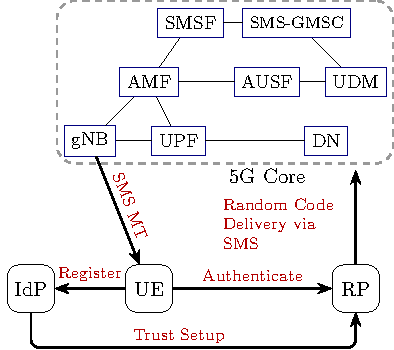
\includegraphics[width=6cm]{architecture}
	\caption{Architecture of the 2-Factor Authentication System}\label{fig:model}
\end{figure}

\subsection{Architectures}
\subsubsection{IdP (Identity providers)}
They are responsible for issuing credentials for other entities, like UE. In this paper, each credential claims a set of attributes, with the signature of the issuing IdPs. 

For different deployment models, a credential can be signed by a single, or multiple IdPs. The latter is more convenient from the perspective of both privacy and reliability. In later content, the construction is described as the one-IdP model, whereas, the extension to the multiple-IdP is straightforward.

\subsubsection{RP (Relying parties)}
They publish diverse services in the network platform. Each service can be accessed according to the RP's designated access policy $\mathcal{P}$. A policy is a predicate, containing a set of attribute values (or value ranges).

In a multi-IdP system, RP only accepts the UE, whose credential satisfies its policy, and signed by its trusted IdPs. Thus, RP will initialize trust relationship between IdPs.

\subsubsection{UE (User equipment)}
It is a concept in 3GPP system, which is an entity with mobile equipment (ME, generally the smart phones) and the USIM card. It can access two network: one the one hand, it can access data network (DN) via 5G data plain (as shown in Fig. \ref{fig:model}) or via other communication technology (e.g., WiFi); on the other hand, it accesses the network services directly provided by the 5G core systems, such as short message services (SMS), voice calls.

As each UE is owned by a user, it will register and request credential from some IdPs, with which, it can proves its privilege to the RPs to enjoy the services in the network. 

\subsubsection{5G Core}
It is a set of network elements provided by a network service provider (NSP). Readers who are interested in it can refer to 3GPP TS23.501 \cite{3gpp23501} to see the entire architecture, and Fig. \ref{fig:model} shows some of them, which relate to our construction. Especially, the UDM is in the domain of home agent, maintaining UE's subscription and context data; AMF is a core element for controlling plane; SMSF and SMS-GMSC are elements specific for short message services. Table \ref{tab:5G} depicts a more detailed introduction.

Return to the system model, the 5G core system is responsible for short message delivery for UE, to assist the multi-factor authentication between diverse RPs. It also has ability to undertake package relay for UE's Internet tasks.%, whereas, it is optional.

\begin{table}[t]
	\caption{Necessary Description for 5G Core}\label{tab:5G}
	\centering
	\begin{tabular}{c|p{6cm}}
		\hline
		\textbf{Notations} & \textbf{Description} \\
		\hline
		AMF & Access and Mobility Management Function, it supports necessary controlling plane signals, e.g., device authentication, paging, and SMS over NAS.\\
		UDM & Unified Data Management, a core element to maintain each UE's in order to realize network and security services.\\
		SMSF & Short Message Service Function, it supports SMS over NAS, delivering messages between UE and SMS-GMSC, IWMSC, or SMS-Routers.\\
		UPF & User Plane Function, it can be seen as a gateway to exchange Internet packets from data network (DN).\\
		MSI-SDN & Mobile Subscriber International ISDN number is a unique and immutable phone number of a UE.\\
		\hline
	\end{tabular}
\end{table}

%The protocol involves the following entities - the user, the relying party (RP), the issuer, and the 5G system network. Each of the roles are described below:
%\begin{list}{}{}
 %   \item{\bf{User/Prover:}} The user is equipped with a mobile phone that supports 5G communication and wants to access to different services provided by various service providers. To this goal, the user retrieves an sttribute-based anonymous credential from the Issuer, and registers for the SMS-relay service at the 5G system network prior to the authentication.
  %  In the authentication phase, the user requires access to resources provided by a third relying party by passing a 2-factor authentication which proves its validity. \\
   % \item{\bf{Relying Party (RP)/Verifier:}} RP is a third party application that the user requires access to. It performs the user authentication by validating user's knowledge of anonymous credential and possession of mobile phone (through SMS verification).\\
    %\item{\bf{Issuer/Identity Provider (IdP):}} The issuer creates credential for a user by executing the issuance protocol. It also defines the general parameters that all parties in the anonymous credential system (Issuer, Verifer and Prover) must agree on. The issuer generates a secret-public key pair for the issuance of attribute-based credentials and its verifivation. It only interacts with users who want to acquire a credential, and doesn't participate in the subsequent steps.\\
    %\item{\bf{5G system network:}} The 5G system accepts user's registration for an SMS-relay service for the privacy-preserving authentication of registered user's ownership factor (the mobile phone). \\
%\end{list}


\subsection{Trust Assumption and Security Requirement}

\textbf{IdPs} are totally trust from the perspective of credential business, they honestly issue credential to each UE, according to its precise attributes (e.g., MSI-SDN). However, as has mentioned before, they are curious of UE's private information and likely to track UE's behaviors for any purpose. 

\textbf{RP} is curious of the user's private information. Focusing on the authentication and access control, necessary attributes are required to convince the RP that the UE has the privilege of the service; whereas, it is not allowed to leak unnecessary attribute information to the RP. 

\textbf{UE} is assumed malicious and insecure. On the one hand, an unauthorized UE tries to forge an authentication message for illegal privilege with any feasible means. On the other hand, any stored data (including the valuable credential) are potential to be compromised by adversaries. But it is assumed that the USIM module is a trusted environment. 
%Especially, when taking into account the mechanism of pseudo-random number

\textbf{5G Core} system is a trust network service provider, especially the control plain. All signals between the network elements are confidentially and integrally protected with TLS protocols. The data are stored, transmitted and deleted strictly according to the privacy policy rules.
% Collecting these information may help the relying party to provider better services, but may also be damageable to user's privacy. Therefore, a service provider may try to acquire additional information about the user during the authentication process, or try to track user's behaviors by linking user's different actions.

Hence, the following security aspects are required in this paper.

\begin{itemize}
	\item \textit{Authentication Soundness.} 
	The authentication is multiple factors, meaning that it can be verified only when the UE owns the legal credential for the accessing policy, and at the same time, the MSI-SDN of UE is trustful and reachable. Additionally, two factors cannot collude to accomplish an authentication between two owners.
	\item \textit{Fine-Grained Access Control.} The access control should be arbitrarily described as an accurate access predicate over a set of attributes.
	\item \textit{Privacy Preserving.} Apart from the necessary information for the access control, private information 
	\item \textit{Semi Accountability.} For services with real-name and traceability requirements, the following property is defined, without sacrificing any privacy 
\end{itemize}

\begin{definition}[Semi Accountability]
	For a same service $RID$ published by one RP, a UE with one MSI-SDN $m_t$, since the only approach for an RP to associate two authentication is by the pseudo-random number $pm$ (as to be proved in Section \ref{sec:xxx}), the accountability is preserved if the adversary UE cannot forge two different pseudo-random numbers $pm_0\neq pm_1$, such that for $i\in (0,1)$
	\begin{align}
	\mathcal{V}(\pi_i) = 1, \pi_i = (m_t|pm_i\gets\mathcal{G}(m_t, RID))
	\end{align}
	where, $\pi(x|\mathcal{L}(x, <y>))$ denotes a proof for mastering a secret $x$, which proves that $x$ can formulate a predicate $\mathcal{L}$ with a set of public parameters $<y>$; $\mathcal{G}$ is a collision-resist one-way generation function; and the output of $\mathcal{V}$ denotes whether the proof can be convinced successfully.
\end{definition}

A scheme could be considered secure if it satisfies the following security goals:
\subsubsection{Completeness}
The user executes the complete procedure of the multi-factor authentication protocol with the relying party, and no additional private information is leaked in the process.
\begin{list}{}{}
    \item{\bf{Multi-factor authentication: }}
    \item{\bf{Privacy-preserving: }}The privacy preservation of our scheme mainly focuses on the following problems: 1) the selective disclosure of attributes, which means that the user can choose to disclose only part of its credential attributes to the third party service provider. This allows the user to de-identify itself as much as possible in the authentication process, and enables the service provider to implement fine-grained access control. 2) The unlinkability of a user's authentication behavior with different service providers. 3) The hiding of the virtual mobile phone. And the existence of external adversaries or dishonest agents should also be taken into consideration.\\
    \item{\bf{Intra-service linkability: }}This feature has nothing to do with the privacy protection of user information. We take it into consideration because we hope that the same user's action with the same service provider could be traceable, so that it would be possible for the service provider to handle the problem of tracing to the source of rumors and its management and control.\\
\end{list}

\section{Construction}
In this section, we go through an entire authentication process to show the whole flow path of our protocol. To get authenticated, the system goes through four steps: of the initial system setup, the SMS-service registration, the credential issuance, and 2-factor authentication. The notions used for the protocol description are used in table 1.
%moved here for pagination purposes
\begin{table}[!ht]
\begin{center}
\caption{Notions Used For Protocol Description.}
\label{tab1}
\begin{tabular*}{\columnwidth}{|c|p{5.45cm}|}
\hline
\textsc{Symbol} & \centerline{\textsc{Description}}\\
\hline
$\mathrm{S}$ & Credential schema defined by identity provider, defines the number of attributes aggregated in the credential and their corresponding meanings.\\
$n$ & Attribute dimension of the credential issued by identity provider.\\
$\left\{M_{i}\right\}_{i \in[[1, n]]}$ &
Attribute messages sent by the user to the IdP to acquire its credential.
\\
$\left\{m_{i}\right\}_{i \in[[1, n]]}$ &
Attribute values of user converted from $\left\{M_{i}\right\}_{i \in[[1, n]]}$ so that $m_i \in \mathbb{Z}_p$
\\
$t\in [[1, n]]$& The index of the attribute that corresponds to user's real mobile phone number. \\
$M_t(MSISDN), m_t$ & User's real mobile phone number and the corresponding attribute value.\\
$pm$ & Virtual mobile phone number generated by the user for a unique 
relying party.\\
$H_1, H_2, H_3, H_4$ & Four secure cryptographic hash functions that the whole system agrees on.\\
$RID$ & Unique identifier assigned to relying party.\\
$A_d, A_h$ & Set of attribute indexes to be disclosed/hidden, where $A_d$ is defined by relying party's access policy.\\
$\mathcal{M}_d, \mathcal{M}_h$ & Set of user's attribute values to be disclosed/hidden. \\
\hline 
\end{tabular*}
\end{center}
\end{table}
\subsection{System Setup}
In the setup phase, the following algorithms are executed in order only once for the bootstrapping of the identity provider. 
\begin{list}{}{}
    \item{\bf{Setup($1^{\lambda}$)$\rightarrow$($para$): }} Output \textsf{Cred.Setup($1^\lambda$)}.\\
    \item{\bf{KeyGen($para$)$\rightarrow$($sk, pk$): }}Output \textsf{Cred.KeyGen($para$)}. Run by the IdP to generate its private-public key pair $(sk, pk)$ from $para$.\\    
\end{list}
At the end of the setup phase, the public parameters ($para, pk$) of the identity provider should be generated and published to whole system. Apart from that, any relying party that has joined the system should be assign a unique identifier $RID$ and publish its access policy, which then defines $A_d$.
\subsection{Credential Issuance}
The following algorithm is executed periodically by the issuer, when a new user acquires a credential from the identity provider (issuer).
\begin{list}{}{}
    \item{\bf{Issue($pp, sk, \mathcal{M}$)$\rightarrow$($\sigma$): }} Output \textsf{Cred.Issue($pp, sk, \mathcal{M}$)}. The interactive algorithm is executed between the user who wants to acquire an attribute-based anonymous credential and the credential issuer. As a result of the execution, the credential $\sigma$, embedded with the user attributes $\mathcal{M}$, is sent to user through a secure channel.
\end{list}
\subsection{SMS-relay registration}
We describe the algorithm implementing the SMS-relay service registration phase; the algorithms are executed each time a user tries to authenticate with and get access to a new service provider.
\begin{list}{}{}
    \item{\bf{Prove1($H_1, H_2, H_3, p, RID, m_t, s$)$\rightarrow$($\Theta_1$): }}
    pick two randoms $r_t$ and $r_0$ from $\mathbb{Z}_p$ and compute $$R\rightarrow H_1(RID)^{r_t}\cdot H_2(RID)^{r_0}.$$
    
    Run by the user to construct a proof $\Theta_1$ proving that it knows the real mobile phone number $m_t$ and the secret parameter $s$, and that the virtual number $pm$ is generated based on $(RID, m_t, s)$.
\end{list}
\subsection{Two-Factor Authentication}

\section{Analyse}
\subsection{Security Analysis}
\subsubsection{Completeness}
We first prove the completeness of the procedure: if the user is honest, and holds an attribute-based anonymous credential $\sigma=(A, x, s)$, then it is able to pass the authentication if it correctly executes all the required steps.
%\begin{list}{}{}
 %   \item{\bullet}If the user is honest, and possesses a credential $\sigma$ 
%\end{list}

\subsection{Efficiency}


\bibliographystyle{plain}
\bibliography{content/citation}
%%%%%%%%%%%%%%%%%%%%%%%%%%%%%

%\section{Introduction}

%% Background of target technology (MFA or authentication, or cryptographic authentication, or anonymous credential)
\IEEEPARstart{T}{he} advances in network technologies from the architecture (e.g., 5th-generation network, Internet of Things) has resulted in the continuous growth in the numbers of connected smart devices through the Internet, which brings in larger and larger market for organizations and enterprises to provide up-layer network services. As these services trend to offer more valuable or private information data (such as personal balance in a bank, private status of the owner's house), and some services are critical to user's safety (like payment), thus the service should be offered with a well-deployed authentication method to resist various adversaries.
%Large amount of data, possibly relevant to every area of human activity, both public and private, will be produced, communicated, gathered, stored, and processed. To keep the transmitted data safe, authentication acts as the first line of defence against adversaries.

According to [], through the process of authentication, a security system validates whether a user could be granted the corresponding access privilege. Based on the authentication mechanism used, the user provides pieces of evidence (factors) of identity so that the security system is convinced whether the user is who it claims to be, or belongs to a certain legitimate user group. Depend on the specific evidence submitted by the user, authentication factors could be categorized into three groups: knowledge factors, ownership factors, and inherent factors. The knowledge factor is something that only the user knows, such as its password or secret key. The possession factor is something that a user has, such as smart cards or mobile phones. The inherent factor refers to something that qualifies a user, such as biometric data. 
%The location factor refers to somewhere the user is, such as current location or time information. 
In some cases, authentication mechanisms could be integrated with cryptography-defined concepts to expand various functions. For example, the cryptographic challenge-response based authentication protocol is an improvement to privacy of the basic password authentication protocol in terms of brute force and dictionary attacks; By employing attribute-based cryptographic framework, one can realize fine-grained access control of data and resources; The anonymous credential system provides privacy-preservation for user attributes and behaviors and unlinkability under a single sign-on framework. 

``Authentication technologies can both advance and undermine privacy interests'' (National Research Council. 2003). An authentication system may require users to reveal identifying personal information to prove their validity, and the act of authentication itself may be recorded and linked with other user behaviors, causing privacy concerns \cite{national2003goes}. Instead of revealing identifiable information, privacy-concerned users may hope to finish authentication step with a service provider only by showing user's belonging to a valid group or by proving its possession of some specific attribute identifiers\cite{holt2002selective}. Anonymous credential system (ACS) is an effective solution to problem of linkability. Users are known to service providers by pseudonyms in such systems, which ensures the anonymity and unlinkability of authentication[]. In addition, ACS enables privacy-preserving single sign-on (SSO)[]. In traditional SSO, a third party identity provider (IdP) serves as single point of failure; And users are at risk of having their activities tracked by the IdP. On contrary, the process of user authentication no longer depends on a single trusted third party in privacy-preserving SSO[]. In []'s work, the anonymous credential system (ACS) is extended to an attribute-based anonymous credential system (ABACS). Compared to ACS, ABACS enables flexible attribute-based access control and minimal disclosure of information, and is thus welcomed by privacy-concerned users.

Key-based (cryptographic) authentication exhibits fragility in the face of key compromise attacks. Multi-factor authentication overcomes this risk. By requiring more than one factor to authenticate a user, the multi-factor authentication (MFA) makes the intruding process more difficult for hackers, thus providing additional layers of security. For example, MFA used on top of username/password authentication may require users to take an extra step such as entering a code sent to a physical device. Even if the perpetrator brute forces the password, it is not able to get pass the second authentication step without possession of the device. Up till now, few researches has been made on the implementation of ABACS with MFA. The popularization of smartphones has lead to increased usage of short message service (SMS) based multi-factor authentication. In these days, most internet applications require users to accomplish the SMS authentication step to get registered or authenticated, making combination user-friendly. However, one concern is that SMS authentication requires users to transmit their personal information to the service provider, including the user's mobile phone number, which identifies a user's identity better than its real name in today's world. Besides, using the same phone number for each authentication risks damaging the unlinkability provided by ABACS. 

\subsection{Our Contribution}

To address the above problems, we construct a multi-factor authentication scheme that combine attribute-based anonymous credential system with SMS-verification code authentication which employs virtual mobile phone number to protect user privacy. We alter the 5G signalling so that a user who has registered for an SMS-relay service at the 5G system network with a virtual mobile phone number could receive the SMS-verification code on its own mobile phone. When the user wants to authenticate with a service provider (SP), it sends to SP information unique to the user with the mobile phone number replaced by a virtual one. Subsequently, the user's phone number is never transmitted onto the internet.

Our scheme realizes an asynchronous SSO system based on an attribute-based anonymous credential framework. The generation of the material for authentication (the attribute-based credential and related information) is decoupled in time with the process of user's authentication at service provider. Hence relying party (the service provider) no longer has to visit the IdP for identity verification. The IdP could be offline while the authentication process running smoothly, and the tracking of user's activities by IdP is prohibited. The ABACS and the employment of virtual mobile phone number provides solid anonymity and unlinkability.

For many online services, intra-service unlinkability is undesirable. If the generation and registration of virtual phone number is arbitrary, a user may have unlimited number of pseudonyms without restriction. 
In our scheme, the generation of virtual mobile phone number and its registration at the 5G system network are designed to be bounded by the unique identifier of the target service provider.
The user could generate multiple virtual numbers once it has acquired an attribute-based credential, but could not generate and register more than one for the same service provider. 




% If a user consistently uses the same identifier, whether it is a real identity or an anonymous one, to participate in transactions with multiple service providers, it risks exposing its behavioral privacy to the outside. The protection of behavioral privacy has become an important topic in information security. In the age of big data, it is technically possible to accurately analyze users' preferences and interests after mining a large amount of users' continuous behaviors, and to predict the future behavior of users with high accuracy. More dangerously, if an adversary already has acquired a part of the behavior information of an observed entity, and compares it with the behavior data of a de-identified identity, the identity of all behaviors of the user may be recovered, which means that the identity privacy of users would be affected to a certain extent. A core requirement to protect behavioral privacy is to achieve unlinkability in multiple user authentications. That is, if two authentication requests are collected, there is no way to tell whether the two requests are from the same user. In our scheme, inter-service unlinkability is desired. The cancellation of interaction with IdP in the authentication process prevents the IdP from tracking user's activities and different RPs. In addition to this, we hope that the correlation of user's authentication with different RPs should be impossible for any other entities in the system. This implies the unlinkability between user's generated random mobile phone numbers for differents RPs and the unlinkability between the assertion constructed by the user for different RPs.


%Network technologies have been advancing rapidly in recent years from the architecture to the up-layer services, such as fifth-generation (5G) radio network and Internet of Things (IoT). The service-based architecture of 5G network and network slicing technique make it easy to converge high-throughput MBB, low-delay IoT and "ultra-reliable low latency communications (URLLC)" into one system, which significantly increase the development of network-dependent technologies\cite{zanella2014internet}. The number of connected devices in the world is expected to exceed 27 billion by 2025\cite{numberconnectediotdevices}. While the paradigm fosters services of convenience in various domains, it should be noted that the pervasive nature of the information sources means that a large amount of data, possibly relevant to every area of human activity, both public and private, will be produced, communicated, gathered, stored, and processed\cite{bonetto2012secure}. In this context, network  security problems will bring about greater threats and heavier losses, especially for organizations operating in healthcare, finance, etc\cite{katrenko2022IoT}. To protect against threats from internet adversaries, authentication has become a necessity. Through authentication, entities using online communication could verify whether the entity they are interacting with is honest or not. In doing this, authentication assures secure systems, secure processes and enterprise information security\cite{5shacklett2022authentication}. 
%To get authenticated, the common practice is that the user provides some sort of login credential to an authentication process for it to decide whether to grant of deny user's access. The credential supplied by the user is what is called the authentication factor\cite{6sharmasecurity}. Basically, authentication factors can be divided into the following three categories: 1) knowledge factor (something you know, e.g. password), 2) possession factor (something you have, e.g. smart cards), 3) inherent factor (something associated with who you are, e.g. fingerprints, retina, voice). Other methods involve attribute-based authentication based on information about users and location based factors\cite{6sharmasecurity}\cite{7alqahtanitechnical}. Examples of traditional authentication technologies include username-password challenge, Authentication And Key Agreement (AKA) protocol, Public Key Infrastructure (PKI) -based authentication, and internet security protocols such as IPsec, TLS, etc. Newly emerging or under-research methods include Identity-based Cryptography (IBC) -based authentication and biometric authentication such as fingerprint, iris scan, etc. Among these methods, cryptographic authentication (also known as Key-based authentication, uses cryptographic keys in a challenge-response handshake to prove one's identity\cite{8keybasedauthentication2022}) is capable of providing various services based on different usage scenarios, e.g. fine-grained access control and privacy-preservation by employing anonymous credentials and attribute-based encryption\cite{9goyal2006attribute, 10guo2014anonymous}. However, key-based authentication exhibits fragility in the face of key compromise attacks\cite{solomon2021how}. To tackle the problem, Multi-factor authentication is called on to provide a boost to security: it is stated that MFA can block over 99.9 percent of account compromise attacks\cite{11onesimpleaction2019}. MFA makes the intruding process more difficult for hackers by providing additional layers of security. For example, MFA used on top of username/password authentication may require users to take an extra step such as entering a code sent to a physical device. Even if the perpetrator brute forces the password, it is not able to get pass the second authentication step without possession of the device.

%''Authentication technologies can both advance and undermine privacy interests" (National Research Council. 2003). An authentication system may require users to reveal identifying personal information to prove their validity, and the act of authentication itself may be recorded and linked with other user behaviors, causing privacy concerns\cite{national2003goes}. Instead of revealing identifiable information, users hope to finish authentication step with a service provider only by showing user's belonging to a valid group or by proving its possession of some specific attribute identifiers\cite{holt2002selective}. Anonymous credential credential is an effective solution to these requirements. With the help of zero-knowledge proof, attribute-based authentication and access control between user and service provider could be achieved while minimizing personal information release\cite{camenisch2002design}. 

%A drawback of anonymous credential is that potential leakage of credentials may lead to identity misuse, which makes anonymous credentials unsuitable for real e-commerce applications and web services that require high security level and strong identifiers\cite{bertino2008security}. Such problem could be addressed by combining anonymous credential with other authentication factors to provide multi-factor authentication. However, the other authentication factor should be chosen with caution. First, a cyptography-based authentication factor is not recommended, as it faces the same drawback as that of the anonymous credential. Such combination of authentication factors has no effect in promoting each other in different security aspects. Second, as has mentioned in the previous paragraph, trivial authentication factors may lead to a breach of privacy protection provided by anonymous credential.


%The analysis of authentication and security protocols involves thorough debugging of the protocol to prove that no flaws could be abused by adversaries or dishonest users to obtain or alter vital information. Such analysis is only possible by using formal techniques\cite{mao1993towards}. Various formal analysis tools have been developed for modeling and performing mathematical analysis on cryptography-based security protocols, such as Scyther, ProVerif, Tamarin-Prover, etc\cite{cremers2008scyther, blanchet2018proverif, meier2013tamarin}. 


%\section{Our contribution}
%In this paper, we present a two-factor credential-based authentication scheme. Our scheme provides strong privacy protection and fine-grained access control. Users could choose to disclose only a part of the attributes in the credential to the relying party, and the relying party could define different access policies requiring different combination of attributes. Our authentication scheme improves the security level by employing a second mobile phone-based authentication factor. By sending to RP a verification code previous received through SMS, the user is able to prove its possession of the mobile phone, which is simple for operation and effective. A virtual mobile phone number generation method is designed with an SMS relying service on the 5G core such that users could hide their real mobile phone number from the internet. The unlinkability of the authentication process is also ensured. Our scheme also features asynchronous single sign-on. The generation and issuance of user's anonymous credential at the identity provider (IdP) is time-decoupled from the user authentication procedure, therefore the IdP needn't always be online. Our scheme realizes a real-name system, in which a user could not cheat the RP into believing it if it has been marked as malicious. In the end, we provide a formal security proof using the tool for formal proof Tamarin-prover to demonstrate that the proposed authentication scheme indeed enforces its security guarantees.
%\input{template/The Design Intent, and Limitations of the Templates}
%\input{template/Where to Get LaTeX Help --- User Groups}
%\input{template/Other Resources}
%\input{template/Text}
%\input{template/Some Common Elements}
%\input{template/Tables}
%\input{template/Algorithms}
%\input{template/Mathematical Typography and Why It Matters}
%\input{template/Conclusion}
%\input{template/Acknowledgements}
%\input{template/end.tex}

















\end{document}


